\documentclass[aspectratio=169,10pt]{beamer}
\usetheme{Madrid}
\usecolortheme{seahorse}

\usepackage{amsmath,amssymb,amsfonts}
\usepackage{mathtools}
\usepackage{xcolor}
\usepackage{listings}
\usepackage{graphicx}
\usepackage{array}
\usepackage{xfrac}
\usepackage{fancybox}

\setbeamertemplate{footline}[frame number]
\setbeamertemplate{navigation symbols}{}

\graphicspath{{figures/}}

% Code styling
\lstset{
    language=Python,
    basicstyle=\ttfamily\scriptsize,
    keywordstyle=\color{blue}\bfseries,
    commentstyle=\color{green!50!black}\itshape,
    stringstyle=\color{red},
    breaklines=true,
    frame=single,
    numbers=left,
    numberstyle=\tiny,
    stepnumber=1,
    showstringspaces=false,
    tabsize=2
}

\title{Variational Inequality Problems}
\subtitle{Section 7.4: Mappings Associated with Variational Inequality}
\author{Based on Pathak's Introduction to Nonlinear Analysis}
\institute{Fixed Point Theory \& Optimization Course}
\date{\today}

\begin{document}

\frame{\titlepage}

% ============================================================================
% TABLE OF CONTENTS
% ============================================================================

\begin{frame}
\frametitle{Outline}
\tableofcontents
\end{frame}

% ============================================================================
% SECTION 1: INTRODUCTION TO VARIATIONAL INEQUALITY
% ============================================================================

\section{Introduction to Variational Inequality Problems}

\begin{frame}
\frametitle{What is a Variational Inequality?}

\begin{definition}[Variational Inequality Problem]
Let $K$ be a nonempty closed convex subset of $\mathbb{R}^n$ and $F : K \to \mathbb{R}^n$ be a mapping.
The \textbf{variational inequality problem} (VIP) is:

\[
\boxed{\text{Find } \bar{x} \in K \text{ such that } (x - \bar{x})^T F(\bar{x}) \geq 0 \text{ for all } x \in K}
\]
\end{definition}

\vspace{0.3cm}

\begin{itemize}
    \item Fundamental problem in optimization, game theory, and numerical analysis
    \item Unifies fixed point problems, optimization, complementarity, and equilibrium problems
    \item Solution interpretation: $F(\bar{x})$ is ``orthogonal'' to the feasible direction $x - \bar{x}$
\end{itemize}

\vspace{0.3cm}

\begin{block}{Key Classes of VIP}
\begin{itemize}
    \item \textbf{Linear VIP}: $F(x) = Ax + b$ for matrix $A$ and vector $b$
    \item \textbf{Nonlinear VIP}: General nonlinear mapping $F$
    \item \textbf{Monotone VIP}: $F$ is monotone operator
\end{itemize}
\end{block}

\end{frame}

\begin{frame}
\frametitle{Equivalent Formulations of VIP}

\vspace{0.2cm}

\begin{columns}[T]
\column{0.5\textwidth}

\textbf{Original Form:}
\[(x - \bar{x})^T F(\bar{x}) \geq 0 \quad \forall x \in K\]

\vspace{0.3cm}

\textbf{Equivalent Forms:}

1. \textbf{Normal Equation}:
\[0 \in F(\bar{x}) + N_K(\bar{x})\]
where $N_K(\bar{x})$ is normal cone to $K$ at $\bar{x}$.

2. \textbf{Fixed Point Form}:
\[\bar{x} = P_K(\bar{x} - \alpha F(\bar{x}))\]
for some $\alpha > 0$.

\column{0.5\textwidth}

3. \textbf{Normal-Fixed Point Equation}:
\[\Psi_\alpha(x) = 0\]
where
\[\Psi_\alpha(x) = f(P_K((1+\alpha)x\]
\[\quad - \alpha P_K(x - \alpha f(x))))\]
\[\quad + \alpha(P_K(x - \alpha f(x))\]
\[\quad - P_K(x))\]

\vspace{0.3cm}

\textit{These formulations allow us to use}
\textit{different theoretical and computational approaches}

\end{columns}

\end{frame}

% ============================================================================
% SECTION 2: PROJECTION OPERATORS
% ============================================================================

\section{Projection Operators and Their Properties}

\begin{frame}
\frametitle{Projection Operator Definition}

\begin{definition}[Projection Operator]
For a nonempty closed convex set $K \subseteq \mathbb{R}^n$ and point $z \in \mathbb{R}^n$,
the \textbf{projection of $z$ onto $K$} is:

\[
P_K(z) = \arg\min_{y \in K} \|z - y\|^2
\]

i.e., $P_K(z)$ is the unique point in $K$ closest to $z$.
\end{definition}

\vspace{0.3cm}

\begin{figure}
\centering

\includegraphics[width=0.45\textwidth]{fig_projection_operator}
\caption{Projection onto a convex set}
\end{figure}

\vspace{-0.3cm}

\begin{itemize}
    \item \textbf{Existence and Uniqueness}: Always unique for closed convex $K$
    \item \textbf{Geometric Interpretation}: Closest point, orthogonal separation
\end{itemize}

\end{frame}

\begin{frame}
\frametitle{Key Properties of Projection}

\begin{theorem}[Characterization of Projection]
Let $K$ be a nonempty closed convex subset of $\mathbb{R}^n$ and $z \in \mathbb{R}^n$.
Then $x^* = P_K(z)$ if and only if
\[
(z - x^*)^T(y - x^*) \leq 0 \quad \forall y \in K
\]
\end{theorem}

\vspace{0.2cm}

\begin{block}{Important Properties}
\begin{enumerate}
    \item \textbf{Non-expansiveness}:
    \[\|P_K(x) - P_K(y)\| \leq \|x - y\| \quad \forall x, y\]

    \item \textbf{Idempotence}:
    \[P_K(P_K(z)) = P_K(z) \quad \forall z\]

    \item \textbf{Variational Characterization}:
    \[x^* = P_K(z) \iff (x^* - z)^T(y - x^*) \leq 0 \quad \forall y \in K\]
\end{enumerate}
\end{block}

\end{frame}

\begin{frame}
\frametitle{Projection Lemma (Lemma 7.1)}

\begin{lemma}[Projection Lemma]
Let $K$ be a nonempty closed convex subset of $\mathbb{R}^n$. For any $z \in \mathbb{R}^n$,
we have

\[
(x - P_K(z))^T(P_K(z) - z) \geq 0 \quad \forall x \in K
\]
\end{lemma}

\vspace{0.3cm}

\begin{block}{Proof Sketch}
If $z \in K$, then $P_K(z) = z$ and the inequality is trivial.

If $z \notin K$, by the projection characterization:
\[\|P_K(z) - z\|^2 = (P_K(z) - z)^T(P_K(z) - z) \leq (x - z)^T(P_K(z) - z) \quad \forall x \in K\]

The direction $P_K(z) - z$ is perpendicular to the supporting hyperplane at $P_K(z)$.
Therefore, it makes an obtuse angle with any inward direction from $P_K(z)$ to $x \in K$.
\end{block}

\vspace{0.2cm}

\begin{figure}
\centering
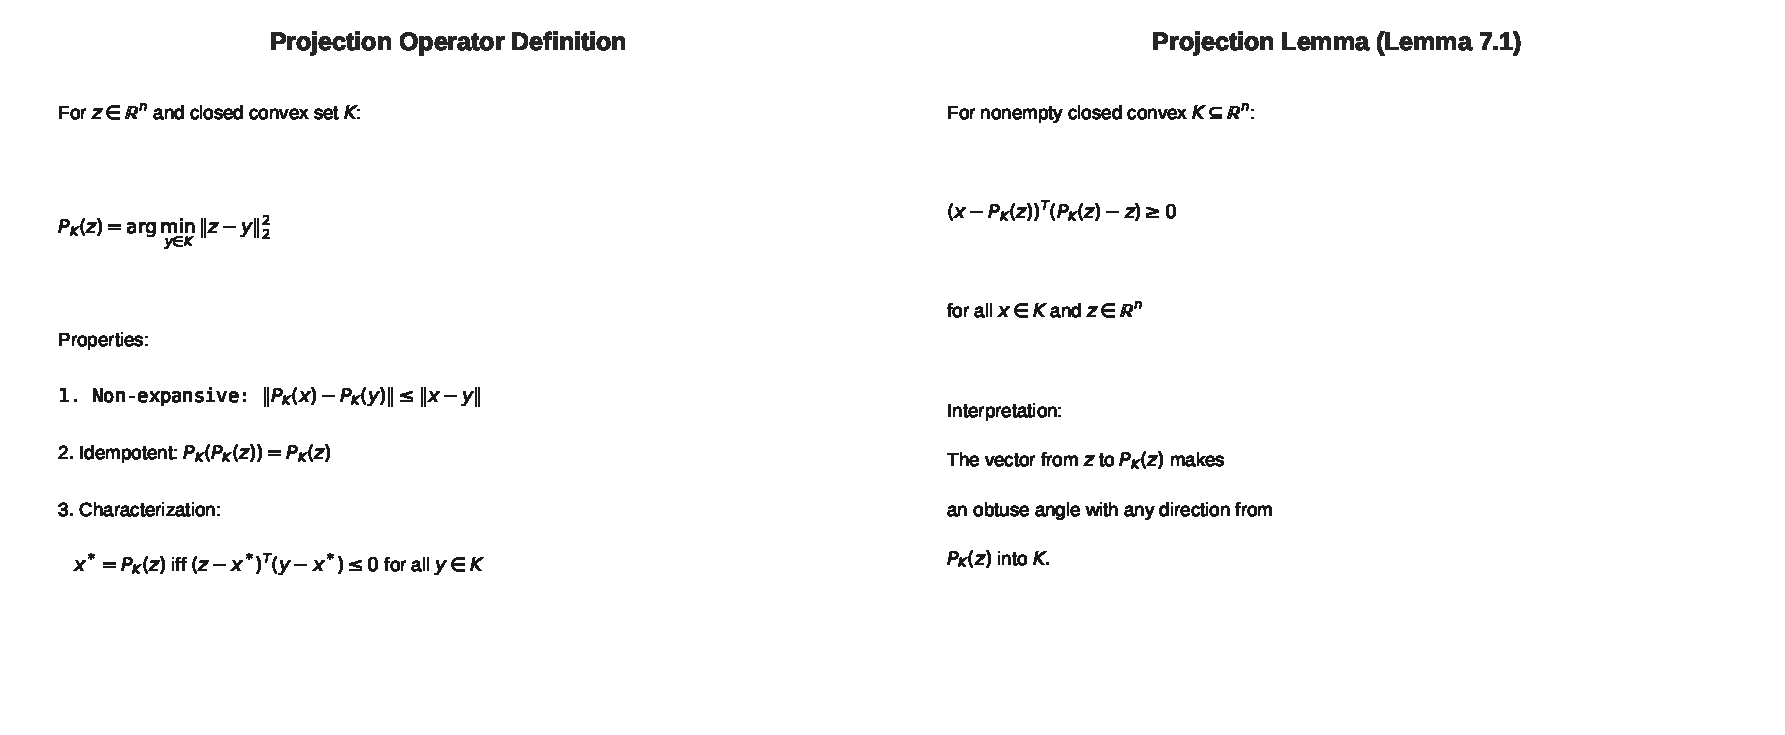
\includegraphics[width=0.35\textwidth]{fig_projection_properties}
\end{figure}

\end{frame}

% ============================================================================
% SECTION 3: NORMAL CONES AND VARIATIONAL INEQUALITIES
% ============================================================================

\section{Normal Cones and VIP Equivalence}

\begin{frame}
\frametitle{Normal Cone and VIP}

\begin{definition}[Normal Cone]
Let $K \subseteq \mathbb{R}^n$ be a nonempty closed convex set and $\bar{x} \in K$.
The \textbf{normal cone} to $K$ at $\bar{x}$ is

\[
N_K(\bar{x}) = \{z \in \mathbb{R}^n : (x - \bar{x})^T z \leq 0 \quad \forall x \in K\}
\]

If $\bar{x} \notin K$, then $N_K(\bar{x}) = \emptyset$ by convention.
\end{definition}

\vspace{0.3cm}

\begin{theorem}[VIP via Normal Cone]
Let $F : K \to \mathbb{R}^n$ be a mapping. Then $\bar{x}$ solves VIP if and only if

\[
0 \in F(\bar{x}) + N_K(\bar{x})
\]

Equivalently,
\[
-F(\bar{x}) \in N_K(\bar{x})
\]
\end{theorem}

\vspace{0.2cm}

\begin{figure}
\centering

\includegraphics[width=0.45\textwidth]{fig_normal_cone}
\caption{Geometry of VIP: $-F(\bar{x})$ must point into normal cone}
\end{figure}

\end{frame}

\begin{frame}[allowframebreaks]
\frametitle{Example 7.1: Optimization and Normal Cones}

\begin{example}
Let $\psi$ be a $C^1$ function on an open set $\Omega$ containing $K$.
A necessary condition for $k_0 \in K$ to be a local minimizer of $\psi$ on $K$ is

\[
0 \in d\psi(k_0) + N_K(k_0)
\]

where $d\psi(k_0)$ is the gradient of $\psi$ at $k_0$.
\end{example}

\vspace{0.3cm}

\textbf{Connection to VIP}:

\begin{enumerate}
    \item If $k_0$ is a local minimizer of $\psi$ on $K$, then
    \[\text{Find } k \in K \text{ such that } (k - k_0)^T \nabla\psi(k_0) \geq 0 \text{ for all } k \in K\]

    This is a VIP with $F = \nabla\psi$.

    \item The normal equation form: $0 \in \nabla\psi(k_0) + N_K(k_0)$ connects optimization to VIP.

    \item Many optimization problems reduce to solving VIPs.
\end{enumerate}

\end{frame}

% ============================================================================
% SECTION 4: FIXED POINT AND NORMAL-FIXED POINT EQUATIONS
% ============================================================================

\section{Fixed Point Equations and NFP Formulation}

\begin{frame}
\frametitle{VIP as Fixed Point Problem}

\vspace{0.1cm}

\begin{theorem}
Let $\bar{x}$ be a solution to VIP. Then for any $\alpha > 0$,

\[
\bar{x} = P_K(\bar{x} - \alpha F(\bar{x}))
\]

and conversely, if this fixed point equation holds, then $\bar{x}$ solves VIP.
\end{theorem}

\vspace{0.3cm}

\begin{block}{Proof}
Suppose $\bar{x}$ solves VIP. Let $y = \bar{x} - \alpha F(\bar{x})$ for $\alpha > 0$.

For all $x \in K$:
\[(x - \bar{x})^T F(\bar{x}) \geq 0 \quad \Rightarrow \quad (x - \bar{x})^T(\bar{x} - y) = -\alpha(x - \bar{x})^T F(\bar{x}) \leq 0\]

By projection characterization, $\bar{x} = P_K(y) = P_K(\bar{x} - \alpha F(\bar{x}))$.
\end{block}

\vspace{0.3cm}

\begin{figure}
\centering
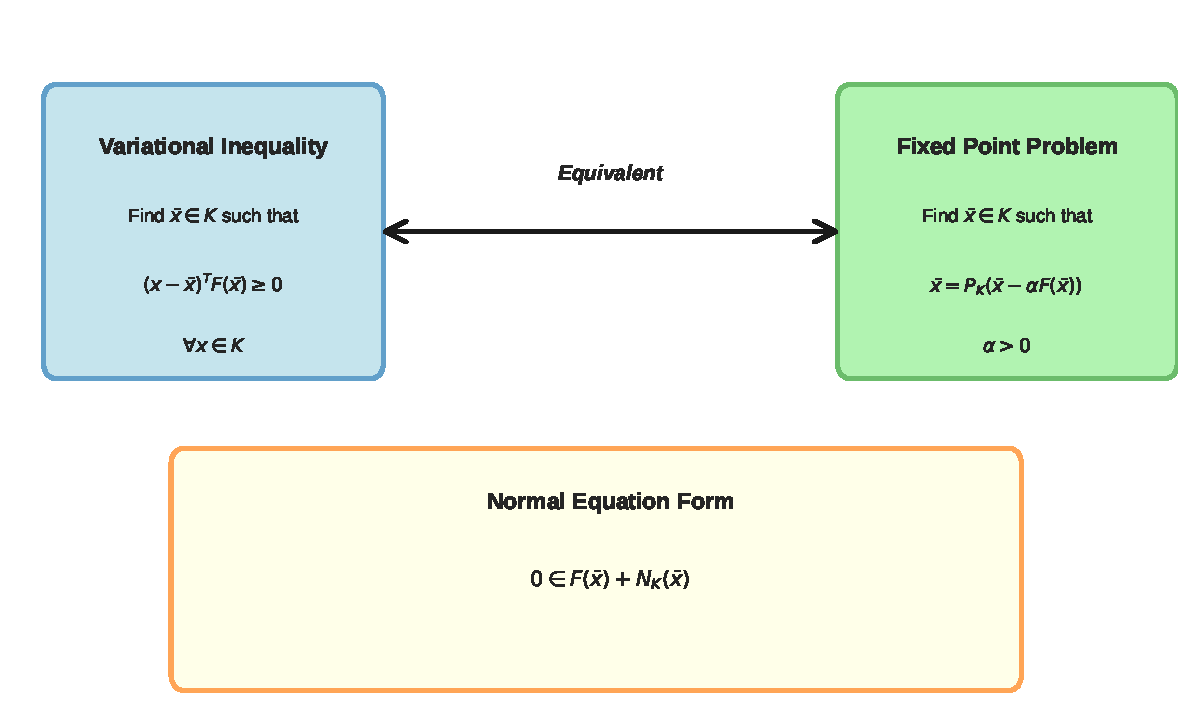
\includegraphics[width=0.55\textwidth]{fig_equivalence}
\end{figure}

\end{frame}

\begin{frame}
\frametitle{Normal-Fixed Point (NFP) Equation}

\vspace{0.1cm}

\begin{definition}[NFP Mapping]
The \textbf{Normal-Fixed Point (NFP)} mapping is defined as:

\[
\Psi_\alpha(x) = f(P_K((1+\alpha)x - \alpha P_K(x - \alpha f(x))))
\]
\[
+ \alpha(P_K(x - \alpha f(x)) - P_K(x)) = 0
\]

where $\alpha > 0$ is the stepsize parameter.
\end{definition}

\vspace{0.3cm}

\begin{block}{Key Results on NFP}
\begin{enumerate}
    \item $\Psi_\alpha$ combines projection and fixed point operators

    \item If $\bar{x}$ solves VIP, then $\Psi_\alpha(\bar{x}) = 0$

    \item If $\Psi_\alpha(\bar{x}) = 0$, then $\bar{x}$ solves VIP

    \item The mapping is more amenable to iterative algorithms
\end{enumerate}
\end{block}

\vspace{0.2cm}

\begin{figure}
\centering
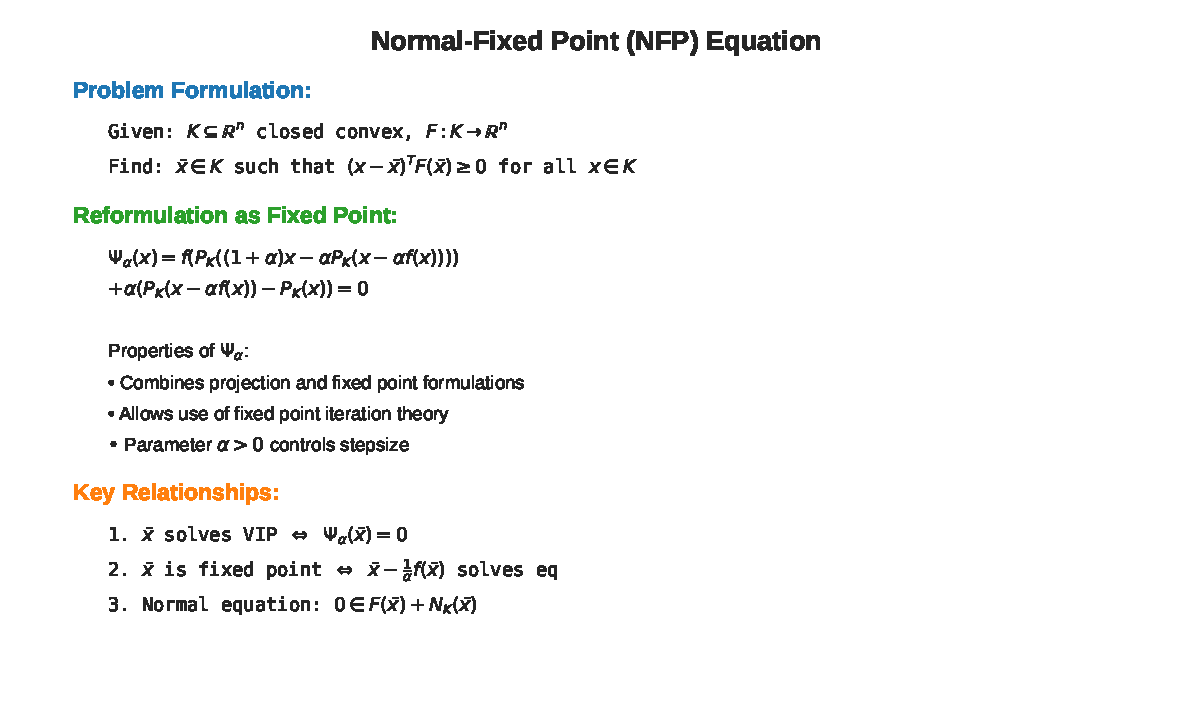
\includegraphics[width=0.5\textwidth]{fig_nfp_mapping}
\end{figure}

\end{frame}

\begin{frame}
\frametitle{Connections Between Formulations}

\vspace{0.2cm}

\begin{columns}[T]
\column{0.5\textwidth}

\textbf{Key Relationships}:

\begin{enumerate}
    \item If $\bar{x}$ solves $\text{VI}(K, F)$, then
    \[\bar{x} - \frac{1}{\alpha}f(\bar{x})\]
    solves a related NFP equation.

    \item Converse: Solutions of NFP lead to solutions of VIP.

    \item The choice of $\alpha$ affects convergence rate.
\end{enumerate}

\column{0.5\textwidth}

\textbf{Theoretical Advantages}:

\begin{itemize}
    \item Use fixed point iteration theory
    \item Apply contraction mapping theorems
    \item Leverage projection properties
    \item Connect to monotone operator theory
    \item Handle constrained optimization
\end{itemize}

\end{columns}

\vspace{0.3cm}

\begin{block}{Computational Significance}
The NFP formulation allows us to use iterative methods like:
\begin{itemize}
    \item Picard iteration: $x_{n+1} = \Psi_\alpha(x_n)$
    \item Mann iteration with projection
    \item Proximal point algorithms
\end{itemize}
\end{block}

\end{frame}

% ============================================================================
% SECTION 5: NUMERICAL ALGORITHMS
% ============================================================================

\section{Numerical Algorithms and Applications}

\begin{frame}
\frametitle{Projected Gradient Algorithm}

\begin{block}{Projected Gradient Method for VIP}
\begin{enumerate}
    \item Choose initial point $x_0 \in K$ and stepsize $\alpha > 0$
    \item For $n = 0, 1, 2, \ldots$:
    \[x_{n+1} = P_K(x_n - \alpha F(x_n))\]
    \item Repeat until convergence
\end{enumerate}
\end{block}

\vspace{0.3cm}

\begin{block}{Convergence Properties}
\begin{itemize}
    \item \textbf{Monotone mappings}: Guaranteed convergence under appropriate step sizes
    \item \textbf{Rate}: Linear (geometric) convergence for strongly monotone $F$
    \item \textbf{Practical}: Simple to implement, uses only projection and gradient
    \item \textbf{Stability}: Non-expansive property ensures stability
\end{itemize}
\end{block}

\vspace{0.3cm}

\begin{figure}
\centering

\includegraphics[width=0.5\textwidth]{fig_algorithm_convergence}
\caption{Convergence of projected gradient algorithm to VIP solution}
\end{figure}

\end{frame}

\begin{frame}[fragile]
\frametitle{Python Implementation: Projected Gradient Method}

\begin{lstlisting}
import numpy as np
from scipy.spatial.distance import cdist

def project_onto_box(x, a, b):
    """Project x onto box K = {y : a <= y <= b}"""
    return np.clip(x, a, b)

def project_gradient_vip(F, K_proj, x0,
                         alpha=0.01, max_iter=1000,
                         tol=1e-6):
    """
    Solve VIP using projected gradient method
    F: mapping
    K_proj: projection onto K
    x0: initial point
    """
    x = x0.copy()
    history = [x.copy()]

    for k in range(max_iter):
        # Gradient step
        Fx = F(x)
        x_new = K_proj(x - alpha * Fx)

        # Check convergence
        if np.linalg.norm(x_new - x) < tol:
            print(f"Converged at iteration {k}")
            break

        x = x_new
        history.append(x.copy())

    return x, history

# Example: Quadratic VIP min (1/2) ||Ax - b||^2 on box
A = np.random.randn(10, 10)
b = np.random.randn(10)
F = lambda x: A.T @ (A @ x - b)

x0 = np.zeros(10)
box_proj = lambda x: np.clip(x, -1, 1)

solution, _ = project_gradient_vip(F, box_proj, x0)
print(f"Solution: {solution}")
\end{lstlisting}

\end{frame}

\begin{frame}
\frametitle{Applications of Variational Inequalities}

\vspace{0.2cm}

\begin{columns}[T]
\column{0.5\textwidth}

\textbf{Optimization}:
\begin{itemize}
    \item Constrained minimization
    \item Quadratic programming
    \item Convex optimization
    \item Nonconvex problems (locally)
\end{itemize}

\vspace{0.2cm}

\textbf{Game Theory}:
\begin{itemize}
    \item Nash equilibrium
    \item Oligopoly models
    \item Traffic equilibrium
    \item Network games
\end{itemize}

\column{0.5\textwidth}

\textbf{Economics}:
\begin{itemize}
    \item Market equilibrium
    \item Complementarity conditions
    \item General equilibrium
    \item Spatial models
\end{itemize}

\vspace{0.2cm}

\textbf{Mechanics}:
\begin{itemize}
    \item Unilateral constraints
    \item Friction problems
    \item Contact mechanics
    \item Elasticity
\end{itemize}

\end{columns}

\vspace{0.3cm}

\begin{block}{Common Problem Classes}
\begin{itemize}
    \item Monotone VI: Solution exists and is unique
    \item Pseudo-monotone VI: Solution exists but may not be unique
    \item Non-monotone VI: May have no solution or multiple solutions
\end{itemize}
\end{block}

\end{frame}

\begin{frame}
\frametitle{Complementarity Problems}

\vspace{0.2cm}

\begin{definition}[Linear Complementarity Problem]
Given matrix $M \in \mathbb{R}^{n \times n}$ and vector $q \in \mathbb{R}^n$, find $z \in \mathbb{R}^n$ such that

\[
z \geq 0, \quad Mz + q \geq 0, \quad z^T(Mz + q) = 0
\]
\end{definition}

\vspace{0.3cm}

\begin{theorem}[LCP as VIP]
The linear complementarity problem is equivalent to the VIP:

\[
\text{Find } z \geq 0 \text{ such that } (w - z)^T(Mz + q) \geq 0 \text{ for all } w \geq 0
\]

where $K = \mathbb{R}^n_+ = \{x : x \geq 0\}$ and $F(x) = Mx + q$.
\end{theorem}

\vspace{0.3cm}

\begin{block}{Interpretation}
Complementarity: Either component is zero or the corresponding inequality is tight.
Useful in optimization, economics, and control theory.
\end{block}

\end{frame}

% ============================================================================
% SECTION 6: THEORETICAL RESULTS
% ============================================================================

\section{Existence and Uniqueness Results}

\begin{frame}
\frametitle{Existence Theorem for VIP}

\begin{theorem}[Existence of VIP Solution]
Let $K \subseteq \mathbb{R}^n$ be a nonempty, closed, and bounded convex set,
and let $F : K \to \mathbb{R}^n$ be continuous.
Then the VIP has at least one solution.
\end{theorem}

\vspace{0.3cm}

\textbf{Proof Idea}:
\begin{enumerate}
    \item Consider the fixed point equation: $\bar{x} = P_K(\bar{x} - \alpha F(\bar{x}))$
    \item The map $P_K(\cdot - \alpha F(\cdot))$ is continuous on compact set $K$
    \item By Brouwer's fixed point theorem, a fixed point exists
    \item This fixed point solves the VIP
\end{enumerate}

\vspace{0.3cm}

\begin{block}{Uniqueness Conditions}
\begin{itemize}
    \item \textbf{Strict Monotonicity}: $F$ strictly monotone $\Rightarrow$ unique solution
    \item \textbf{Strong Monotonicity}: $(x-y)^T(F(x)-F(y)) \geq \mu\|x-y\|^2$ for $\mu > 0$
    \item \textbf{Lipschitz Continuity}: Combined with monotonicity ensures uniqueness
\end{itemize}
\end{block}

\end{frame}

\begin{frame}
\frametitle{Convergence Rates}

\vspace{0.2cm}

\begin{theorem}[Convergence Rate for Monotone VIP]
Suppose $F$ is monotone and Lipschitz continuous with constant $L$.
Under appropriate stepsize $\alpha \in (0, 2/L)$, the projected gradient iteration converges.
\end{theorem}

\vspace{0.3cm}

\begin{block}{Convergence Rates}

\begin{enumerate}
    \item \textbf{Monotone (non-strongly)}:
    \[\|x_n - \bar{x}\| = O(1/\sqrt{n})\]
    (sublinear convergence)

    \item \textbf{Strongly monotone}:
    \[\|x_n - \bar{x}\| = O(e^{-\mu n})\]
    (geometric/exponential convergence)

    \item \textbf{Pseudo-monotone}: Convergence with appropriate modifications
\end{enumerate}

\end{block}

\vspace{0.3cm}

\begin{itemize}
    \item Better convergence rates available with advanced algorithms
    \item Methods like proximal point, forward-backward splitting
    \item Accelerated methods can achieve optimal rates
\end{itemize}

\end{frame}

% ============================================================================
% SECTION 7: SUMMARY AND EXTENSIONS
% ============================================================================

\section{Summary and Extensions}

\begin{frame}
\frametitle{Summary of Key Concepts}

\vspace{0.2cm}

\begin{columns}[T]
\column{0.5\textwidth}

\textbf{Core Theory}:
\begin{itemize}
    \item \textbf{VIP Definition}: Find $\bar{x} \in K$ with $(x - \bar{x})^T F(\bar{x}) \geq 0$

    \item \textbf{Projection}: Unique closest point in $K$

    \item \textbf{Normal Cone}: Characterizes VIP conditions

    \item \textbf{Equivalences}: Fixed point, normal equation, NFP

    \item \textbf{Existence}: Under continuity and compactness
\end{itemize}

\column{0.5\textwidth}

\textbf{Computational Methods}:
\begin{itemize}
    \item \textbf{Projected Gradient}: Simple, general purpose

    \item \textbf{Proximal Methods}: Handles non-smooth terms

    \item \textbf{Splitting Methods}: Decompose into subproblems

    \item \textbf{Acceleration}: Improve convergence rates

    \item \textbf{Asynchronous}: Parallel computing
\end{itemize}

\end{columns}

\vspace{0.3cm}

\begin{block}{Key Takeaways}
VIP is a unifying framework connecting optimization, fixed points, equilibrium,
and complementarity problems. The projection operator and normal cone provide
geometric interpretation and practical algorithms.
\end{block}

\end{frame}

\begin{frame}
\frametitle{Extensions and Further Topics}

\vspace{0.3cm}

\begin{columns}[T]
\column{0.5\textwidth}

\textbf{Theoretical Extensions}:
\begin{itemize}
    \item \textbf{Monotone Operators}: General operator-theoretic framework

    \item \textbf{Inclusion Problems}: $0 \in F(x) + T(x)$ with set-valued $T$

    \item \textbf{Generalized VIP}: Multiple operators and constraints

    \item \textbf{Stochastic VI}: Random perturbations

    \item \textbf{Set-Valued Mappings}: Multivalued operators
\end{itemize}

\column{0.5\textwidth}

\textbf{Advanced Methods}:
\begin{itemize}
    \item \textbf{Primal-Dual Algorithms}: Handle multiple operator terms

    \item \textbf{Coordinate Descent}: Solve component-wise

    \item \textbf{Mirror Descent}: Non-Euclidean geometry

    \item \textbf{Variationally Coherent Methods}: Exploit problem structure

    \item \textbf{Machine Learning}: Stochastic and online variants
\end{itemize}

\end{columns}

\vspace{0.3cm}

\begin{block}{Related Topics in the Course}
\begin{itemize}
    \item Chapter 5: Fixed point theorems (foundational for VIP)
    \item Chapter 6: Monotone operators and subdifferentials
    \item Chapter 7: Variational methods and optimization
    \item Chapter 9: Applications to differential and integral equations
\end{itemize}
\end{block}

\end{frame}

\begin{frame}
\frametitle{References and Further Reading}

\vspace{0.3cm}

\textbf{Key References}:

\begin{enumerate}
    \item Pathak, H. K. (2018). \textit{An Introduction to Nonlinear Analysis and Fixed Point Theory}.
    Springer International Publishing.

    \item Kinderlehrer, D., \& Stampacchia, G. (1980). \textit{An Introduction to Variational Inequalities
    and Their Applications}. Academic Press.

    \item Noor, M. A. (2003). Variational Inequalities and Applications.
    In \textit{Encyclopedia of Mathematical Physics}.

    \item Rockafellar, R. T., \& Wets, R. J.-B. (2009). \textit{Variational Analysis}.
    Springer-Verlag.
\end{enumerate}

\vspace{0.3cm}

\textbf{Online Resources}:
\begin{itemize}
    \item Optimization methods courses (e.g., CMU, Stanford)
    \item Monge-Ampère and PDE variational approaches
    \item Numerical methods literature
\end{itemize}

\end{frame}

\begin{frame}
\frametitle{Exercise: Solving a Simple VIP}

\vspace{0.2cm}

\begin{example}[Quadratic Variational Inequality]
Consider the VIP on $K = [0, 1]^n$:

Find $\bar{x} \in K$ such that $(x - \bar{x})^T A\bar{x} \geq 0$ for all $x \in K$

where $A$ is a positive definite matrix.

\vspace{0.2cm}

\textbf{Tasks}:
\begin{enumerate}
    \item Show that this VIP is equivalent to minimizing $\frac{1}{2}\|Ax - 0\|^2$ on $K$

    \item Implement the projected gradient method

    \item Compare convergence rates for $A$ with different condition numbers

    \item Verify the solution satisfies the VIP conditions
\end{enumerate}
\end{example}

\end{frame}

\end{document}
